% Options for packages loaded elsewhere
\PassOptionsToPackage{unicode}{hyperref}
\PassOptionsToPackage{hyphens}{url}
%
\documentclass[
]{article}
\usepackage{amsmath,amssymb}
\usepackage{lmodern}
\usepackage{iftex}
\ifPDFTeX
  \usepackage[T1]{fontenc}
  \usepackage[utf8]{inputenc}
  \usepackage{textcomp} % provide euro and other symbols
\else % if luatex or xetex
  \usepackage{unicode-math}
  \defaultfontfeatures{Scale=MatchLowercase}
  \defaultfontfeatures[\rmfamily]{Ligatures=TeX,Scale=1}
\fi
% Use upquote if available, for straight quotes in verbatim environments
\IfFileExists{upquote.sty}{\usepackage{upquote}}{}
\IfFileExists{microtype.sty}{% use microtype if available
  \usepackage[]{microtype}
  \UseMicrotypeSet[protrusion]{basicmath} % disable protrusion for tt fonts
}{}
\makeatletter
\@ifundefined{KOMAClassName}{% if non-KOMA class
  \IfFileExists{parskip.sty}{%
    \usepackage{parskip}
  }{% else
    \setlength{\parindent}{0pt}
    \setlength{\parskip}{6pt plus 2pt minus 1pt}}
}{% if KOMA class
  \KOMAoptions{parskip=half}}
\makeatother
\usepackage{xcolor}
\IfFileExists{xurl.sty}{\usepackage{xurl}}{} % add URL line breaks if available
\IfFileExists{bookmark.sty}{\usepackage{bookmark}}{\usepackage{hyperref}}
\hypersetup{
  pdftitle={Chapter 22},
  pdfauthor={Alan T. Arnholt - Modified notes from the Second Edition of Probability and Statistics with R},
  hidelinks,
  pdfcreator={LaTeX via pandoc}}
\urlstyle{same} % disable monospaced font for URLs
\usepackage[margin=1in]{geometry}
\usepackage{color}
\usepackage{fancyvrb}
\newcommand{\VerbBar}{|}
\newcommand{\VERB}{\Verb[commandchars=\\\{\}]}
\DefineVerbatimEnvironment{Highlighting}{Verbatim}{commandchars=\\\{\}}
% Add ',fontsize=\small' for more characters per line
\usepackage{framed}
\definecolor{shadecolor}{RGB}{248,248,248}
\newenvironment{Shaded}{\begin{snugshade}}{\end{snugshade}}
\newcommand{\AlertTok}[1]{\textcolor[rgb]{0.94,0.16,0.16}{#1}}
\newcommand{\AnnotationTok}[1]{\textcolor[rgb]{0.56,0.35,0.01}{\textbf{\textit{#1}}}}
\newcommand{\AttributeTok}[1]{\textcolor[rgb]{0.77,0.63,0.00}{#1}}
\newcommand{\BaseNTok}[1]{\textcolor[rgb]{0.00,0.00,0.81}{#1}}
\newcommand{\BuiltInTok}[1]{#1}
\newcommand{\CharTok}[1]{\textcolor[rgb]{0.31,0.60,0.02}{#1}}
\newcommand{\CommentTok}[1]{\textcolor[rgb]{0.56,0.35,0.01}{\textit{#1}}}
\newcommand{\CommentVarTok}[1]{\textcolor[rgb]{0.56,0.35,0.01}{\textbf{\textit{#1}}}}
\newcommand{\ConstantTok}[1]{\textcolor[rgb]{0.00,0.00,0.00}{#1}}
\newcommand{\ControlFlowTok}[1]{\textcolor[rgb]{0.13,0.29,0.53}{\textbf{#1}}}
\newcommand{\DataTypeTok}[1]{\textcolor[rgb]{0.13,0.29,0.53}{#1}}
\newcommand{\DecValTok}[1]{\textcolor[rgb]{0.00,0.00,0.81}{#1}}
\newcommand{\DocumentationTok}[1]{\textcolor[rgb]{0.56,0.35,0.01}{\textbf{\textit{#1}}}}
\newcommand{\ErrorTok}[1]{\textcolor[rgb]{0.64,0.00,0.00}{\textbf{#1}}}
\newcommand{\ExtensionTok}[1]{#1}
\newcommand{\FloatTok}[1]{\textcolor[rgb]{0.00,0.00,0.81}{#1}}
\newcommand{\FunctionTok}[1]{\textcolor[rgb]{0.00,0.00,0.00}{#1}}
\newcommand{\ImportTok}[1]{#1}
\newcommand{\InformationTok}[1]{\textcolor[rgb]{0.56,0.35,0.01}{\textbf{\textit{#1}}}}
\newcommand{\KeywordTok}[1]{\textcolor[rgb]{0.13,0.29,0.53}{\textbf{#1}}}
\newcommand{\NormalTok}[1]{#1}
\newcommand{\OperatorTok}[1]{\textcolor[rgb]{0.81,0.36,0.00}{\textbf{#1}}}
\newcommand{\OtherTok}[1]{\textcolor[rgb]{0.56,0.35,0.01}{#1}}
\newcommand{\PreprocessorTok}[1]{\textcolor[rgb]{0.56,0.35,0.01}{\textit{#1}}}
\newcommand{\RegionMarkerTok}[1]{#1}
\newcommand{\SpecialCharTok}[1]{\textcolor[rgb]{0.00,0.00,0.00}{#1}}
\newcommand{\SpecialStringTok}[1]{\textcolor[rgb]{0.31,0.60,0.02}{#1}}
\newcommand{\StringTok}[1]{\textcolor[rgb]{0.31,0.60,0.02}{#1}}
\newcommand{\VariableTok}[1]{\textcolor[rgb]{0.00,0.00,0.00}{#1}}
\newcommand{\VerbatimStringTok}[1]{\textcolor[rgb]{0.31,0.60,0.02}{#1}}
\newcommand{\WarningTok}[1]{\textcolor[rgb]{0.56,0.35,0.01}{\textbf{\textit{#1}}}}
\usepackage{longtable,booktabs,array}
\usepackage{calc} % for calculating minipage widths
% Correct order of tables after \paragraph or \subparagraph
\usepackage{etoolbox}
\makeatletter
\patchcmd\longtable{\par}{\if@noskipsec\mbox{}\fi\par}{}{}
\makeatother
% Allow footnotes in longtable head/foot
\IfFileExists{footnotehyper.sty}{\usepackage{footnotehyper}}{\usepackage{footnote}}
\makesavenoteenv{longtable}
\usepackage{graphicx}
\makeatletter
\def\maxwidth{\ifdim\Gin@nat@width>\linewidth\linewidth\else\Gin@nat@width\fi}
\def\maxheight{\ifdim\Gin@nat@height>\textheight\textheight\else\Gin@nat@height\fi}
\makeatother
% Scale images if necessary, so that they will not overflow the page
% margins by default, and it is still possible to overwrite the defaults
% using explicit options in \includegraphics[width, height, ...]{}
\setkeys{Gin}{width=\maxwidth,height=\maxheight,keepaspectratio}
% Set default figure placement to htbp
\makeatletter
\def\fps@figure{htbp}
\makeatother
\setlength{\emergencystretch}{3em} % prevent overfull lines
\providecommand{\tightlist}{%
  \setlength{\itemsep}{0pt}\setlength{\parskip}{0pt}}
\setcounter{secnumdepth}{5}
\ifLuaTeX
  \usepackage{selnolig}  % disable illegal ligatures
\fi

\title{Chapter 22}
\author{Alan T. Arnholt - Modified notes from the Second Edition of \emph{Probability and Statistics with R}}
\date{Last compiled: May 10, 2022 at 09:27:36 AM}

\begin{document}
\maketitle

{
\setcounter{tocdepth}{2}
\tableofcontents
}
\hypertarget{comparing-counts}{%
\section{Comparing Counts}\label{comparing-counts}}

\textbf{Objectives:}

\begin{enumerate}
\def\labelenumi{\Roman{enumi}.}
\item
  Goodness of fit test
\item
  Independence test
\item
  Homogeneity test
\item
  What can go wrong?
\end{enumerate}

\begin{center}\rule{0.5\linewidth}{0.5pt}\end{center}

Many statistical procedures require knowledge of the population from which the sample is taken. For example, using Student's \(t\)-distribution for testing a hypothesis or constructing a confidence interval for \(\mu\) assumes that the parent population is normal. In this section, \textbf{goodness-of-fit} (GOF) procedures are presented that will help to identify the distribution of the population from which the sample is drawn. The null hypothesis in a goodness-of-fit test is a statement about the form of the cumulative distribution. When all the parameters in the null hypothesis are specified, the hypothesis is called simple. Recall that in the event the null hypothesis does not completely specify all of the parameters of the distribution, the hypothesis is said to be composite. Goodness-of-fit tests are typically used when the form of the population is in question. In contrast to most of the statistical procedures discussed so far, where the goal has been to reject the null hypothesis, in a GOF test one hopes to retain the null hypothesis.

\hypertarget{the-chi-square-goodness-of-fit-test}{%
\subsection{The Chi-Square Goodness-of-Fit Test}\label{the-chi-square-goodness-of-fit-test}}

Given a single random sample of size \(n\) from an unknown population \(F_X\), one may wish to test the hypothesis that \(F_X\) has some known distribution \(F_0(x)\) for all \(x\). For example, using the data frame \texttt{SOCCER} from the \texttt{PASWR2} package, is it reasonable to assume the number of goals scored during regulation time for the 232 soccer matches has a Poisson distribution with \(\lambda=2.5\)?

The chi-square goodness-of-fit test is based on a normalized statistic that examines the vertical deviations between what is observed and what is expected when \(H_0\) is true in \(k\) mutually exclusive categories. At times, such as in surveys of brand preferences, where the categories/groups would be the brand names, the sample will lend itself to being divided into \(k\) mutually exclusive categories. Other times, the categories/groupings will be more arbitrary. Before applying the chi-square goodness-of-fit test, the data must be grouped according to some scheme to form \(k\) mutually exclusive categories. When the null hypothesis completely specifies the population, the probability that a random observation will fall into each of the chosen or fixed categories can be computed. Once the probabilities for a data point to fall into each of the chosen or fixed categories is computed, multiplying the probabilities by \(n\) produces the expected counts for each category under the null distribution. If the null hypothesis is true, the differences between the counts observed in the \(k\) categories and the counts expected in the \(k\) categories should be small. The test criterion for testing \(H_0: F_X(x) = F_0(x) \text{ for all } x\) against the alternative \(H_1: F_X(x) \ne F_0(x) \text{ for some } x\) when the null hypothesis is completely specified is

\begin{equation}
\chi_{\text{obs}}^2=\sum_{i=1}^{k} \frac{(O_k - E_k)^2}{E_k},
\label{eq:chiobs}
\end{equation}

where \(\chi_\text{obs}^2\) is the sum of the squared deviations between what is observed \((O_k)\) and what is expected \((E_k)\) in each of the \(k\) categories divided by what is expected in each of the \(k\) categories. Large values of \(\chi_\text{obs}^2\) occur when the observed data are inconsistent with the null hypothesis and thus lead to rejection of the null hypothesis. The exact distribution of \(\chi_\text{obs}^2\) is very complicated; however, for large \(n\), provided all expected categories are at least 5, \(\chi_\text{obs}^2\) is distributed approximately \(\chi^2\) with \(k-1\) degrees of freedom. When the null hypothesis is composite, that is, not all of the parameters are specified, the degrees of freedom for the random variable \(\chi_\text{obs}^2\) are reduced by one for each parameter that must be estimated.

\begin{center}\rule{0.5\linewidth}{0.5pt}\end{center}

\hypertarget{example}{%
\subsubsection*{Example}\label{example}}
\addcontentsline{toc}{subsubsection}{Example}

Test the hypothesis that the number of goals scored during regulation time for the 232 soccer matches stored in the data frame \texttt{SOCCER} has a Poisson \textbf{cdf} with \(\lambda=2.5\) with the chi-square goodness-of-fit test and an \(\alpha\) level of 0.05. Produce a histogram showing the number of observed goals scored during regulation time and superimpose on the histogram the number of goals that are expected to be made when the distribution of goals follows a Poisson distribution with \(\lambda=2.5\).

\hypertarget{solution}{%
\subsubsection*{Solution}\label{solution}}
\addcontentsline{toc}{subsubsection}{Solution}

Since the number of categories for a Poisson distribution is
theoretically infinite, a table is first constructed of the observed
number of goals to get an idea of reasonable categories.

\begin{Shaded}
\begin{Highlighting}[]
\FunctionTok{library}\NormalTok{(PASWR2)}
\FunctionTok{xtabs}\NormalTok{(}\SpecialCharTok{\textasciitilde{}}\NormalTok{goals, }\AttributeTok{data =}\NormalTok{ SOCCER)}
\end{Highlighting}
\end{Shaded}

\begin{verbatim}
goals
 0  1  2  3  4  5  6  7  8 
19 49 60 47 32 18  3  3  1 
\end{verbatim}

Based on the table, a decision is made to create categories for 0, 1, 2, 3, 4, 5, and 6 or more goals. Under the null hypothesis that \(F_0(x)\) is a Poisson distribution with \(\lambda=2.5\), the probabilities of scoring 0, 1, 2, 3, 4, 5, and 6 or more goals are computed with \texttt{R} as follows:

\begin{Shaded}
\begin{Highlighting}[]
\NormalTok{PX }\OtherTok{\textless{}{-}} \FunctionTok{c}\NormalTok{(}\FunctionTok{dpois}\NormalTok{(}\DecValTok{0}\SpecialCharTok{:}\DecValTok{5}\NormalTok{, }\FloatTok{2.5}\NormalTok{), }\FunctionTok{ppois}\NormalTok{(}\DecValTok{5}\NormalTok{, }\FloatTok{2.5}\NormalTok{, }\AttributeTok{lower =} \ConstantTok{FALSE}\NormalTok{))}
\NormalTok{PX}
\end{Highlighting}
\end{Shaded}

\begin{verbatim}
[1] 0.08208500 0.20521250 0.25651562 0.21376302 0.13360189 0.06680094 0.04202104
\end{verbatim}

Since there were a total of \(n=232\) soccer games, the expected number of goals for the six categories is simply \(232 \times \tt{PX}\).

\begin{Shaded}
\begin{Highlighting}[]
\NormalTok{EX }\OtherTok{\textless{}{-}} \DecValTok{232}\SpecialCharTok{*}\NormalTok{PX}
\NormalTok{OB }\OtherTok{\textless{}{-}} \FunctionTok{c}\NormalTok{(}\FunctionTok{as.vector}\NormalTok{(}\FunctionTok{xtabs}\NormalTok{(}\SpecialCharTok{\textasciitilde{}}\NormalTok{goals, }\AttributeTok{data =}\NormalTok{ SOCCER)[}\DecValTok{1}\SpecialCharTok{:}\DecValTok{6}\NormalTok{]), }
        \FunctionTok{sum}\NormalTok{(}\FunctionTok{xtabs}\NormalTok{(}\SpecialCharTok{\textasciitilde{}}\NormalTok{goals, }\AttributeTok{data =}\NormalTok{ SOCCER)[}\DecValTok{7}\SpecialCharTok{:}\DecValTok{9}\NormalTok{]))}
\NormalTok{OB}
\end{Highlighting}
\end{Shaded}

\begin{verbatim}
[1] 19 49 60 47 32 18  7
\end{verbatim}

\begin{Shaded}
\begin{Highlighting}[]
\NormalTok{ans }\OtherTok{\textless{}{-}} \FunctionTok{cbind}\NormalTok{(PX, EX, OB)}
\FunctionTok{row.names}\NormalTok{(ans) }\OtherTok{\textless{}{-}} \FunctionTok{c}\NormalTok{(}\StringTok{" X=0"}\NormalTok{,}\StringTok{" X=1"}\NormalTok{,}\StringTok{" X=2"}\NormalTok{,}\StringTok{" X=3"}\NormalTok{,}\StringTok{" X=4"}\NormalTok{,}\StringTok{" X=5"}\NormalTok{,}\StringTok{"X\textgreater{}=6"}\NormalTok{)}
\NormalTok{ans}
\end{Highlighting}
\end{Shaded}

\begin{verbatim}
             PX        EX OB
 X=0 0.08208500 19.043720 19
 X=1 0.20521250 47.609299 49
 X=2 0.25651562 59.511624 60
 X=3 0.21376302 49.593020 47
 X=4 0.13360189 30.995638 32
 X=5 0.06680094 15.497819 18
X>=6 0.04202104  9.748881  7
\end{verbatim}

\textbf{Hypotheses}--- The null and alternative hypotheses for using the chi-square goodness-of-fit test to test the hypothesis that the number of goals scored during regulation time for the 232 soccer matches stored in the data frame \texttt{SOCCER} has a Poisson \textbf{cdf} with \(\lambda=2.5\) are

\begin{align*}
        H_0&: F_X(x) = F_0(x) \sim \text{Pois}(\lambda=2.5)\text{ for all } x \text{ versus
        }\\
        H_A&:  F_X(x) \ne F_0(x) \text{ for some } x.
\end{align*}

\textbf{Test Statistic:}--- The test statistic chose is \(\chi_{\text{obs}}^2.\)

\textbf{Rejection Region Calculations}---Reject if \(\chi^2_{\text{obs}}>\chi^2_{1-\alpha;k-1}\). The \(\chi^2_{\text{obs}}\) is computed with \eqref{eq:chiobs} in \texttt{R} below.

\begin{Shaded}
\begin{Highlighting}[]
\NormalTok{chi\_obs }\OtherTok{\textless{}{-}} \FunctionTok{sum}\NormalTok{((OB }\SpecialCharTok{{-}}\NormalTok{ EX)}\SpecialCharTok{\^{}}\DecValTok{2}\SpecialCharTok{/}\NormalTok{EX)}
\NormalTok{chi\_obs}
\end{Highlighting}
\end{Shaded}

\begin{verbatim}
[1] 1.39194
\end{verbatim}

\(1.3919402= \chi^2_{\text{obs}}\overset{?}{>}\chi^2_{0.95;6}=12.5915872\).

\textbf{Statistical Conclusion}---The \(p-\)value is \(0.9663469\).

\begin{Shaded}
\begin{Highlighting}[]
\NormalTok{p\_val }\OtherTok{\textless{}{-}} \FunctionTok{pchisq}\NormalTok{(chi\_obs, }\DecValTok{7{-}1}\NormalTok{, }\AttributeTok{lower =} \ConstantTok{FALSE}\NormalTok{)}
\NormalTok{p\_val}
\end{Highlighting}
\end{Shaded}

\begin{verbatim}
[1] 0.9663469
\end{verbatim}

\begin{enumerate}
\def\labelenumi{\Roman{enumi}.}
\item
  Since \(\chi^2_{\text{obs}}=1.3919402\) is not greater than \(\chi^2_{0.95;6}=12.5915872\), fail to reject \(H_0\).
\item
  Since the \(p-\)value = \(0.9663469\) is greater than 0.05, fail to reject \(H_0\).
\end{enumerate}

Fail to reject \(H_0\).

\textbf{English Conclusion}---There is no evidence to suggest that the true \textbf{cdf} does not equal the Poisson distribution with \(\lambda=2.5\) for at least one \(x\).

\begin{center}\rule{0.5\linewidth}{0.5pt}\end{center}

To perform a goodness-of-fit test with the function \texttt{chisq.test()}, one may specify a vector of observed values for the argument \texttt{x=}, and a vector of probabilities of the same length as the vector passed to \texttt{x=} to the argument \texttt{p=}.

\begin{Shaded}
\begin{Highlighting}[]
\FunctionTok{chisq.test}\NormalTok{(}\AttributeTok{x =}\NormalTok{ OB, }\AttributeTok{p =}\NormalTok{ PX)}
\end{Highlighting}
\end{Shaded}

\begin{verbatim}
    Chi-squared test for given probabilities

data:  OB
X-squared = 1.3919, df = 6, p-value = 0.9663
\end{verbatim}

The code below uses base graphics to create a histogram with superimposed expected goals and the result is shown in Figure \ref{fig:histo}.

\begin{Shaded}
\begin{Highlighting}[]
\FunctionTok{hist}\NormalTok{(SOCCER}\SpecialCharTok{$}\NormalTok{goals, }\AttributeTok{breaks =} \FunctionTok{c}\NormalTok{((}\SpecialCharTok{{-}}\FloatTok{0.5} \SpecialCharTok{+} \DecValTok{0}\NormalTok{)}\SpecialCharTok{:}\NormalTok{(}\DecValTok{8} \SpecialCharTok{+} \FloatTok{0.5}\NormalTok{)), }\AttributeTok{col =} \StringTok{"lightblue"}\NormalTok{, }
     \AttributeTok{xlab =} \StringTok{"Goals scored"}\NormalTok{, }\AttributeTok{ylab =} \StringTok{""}\NormalTok{, }\AttributeTok{freq =} \ConstantTok{TRUE}\NormalTok{, }\AttributeTok{main =} \StringTok{""}\NormalTok{)}
\NormalTok{x }\OtherTok{\textless{}{-}} \DecValTok{0}\SpecialCharTok{:}\DecValTok{8}
\NormalTok{fx }\OtherTok{\textless{}{-}}\NormalTok{ (}\FunctionTok{dpois}\NormalTok{(}\DecValTok{0}\SpecialCharTok{:}\DecValTok{8}\NormalTok{, }\AttributeTok{lambda =} \FloatTok{2.5}\NormalTok{))}\SpecialCharTok{*}\DecValTok{232}
\FunctionTok{lines}\NormalTok{(x, fx, }\AttributeTok{type =} \StringTok{"h"}\NormalTok{)}
\FunctionTok{lines}\NormalTok{(x, fx, }\AttributeTok{type =} \StringTok{"p"}\NormalTok{, }\AttributeTok{pch =} \DecValTok{16}\NormalTok{)}
\end{Highlighting}
\end{Shaded}

\begin{figure}

{\centering 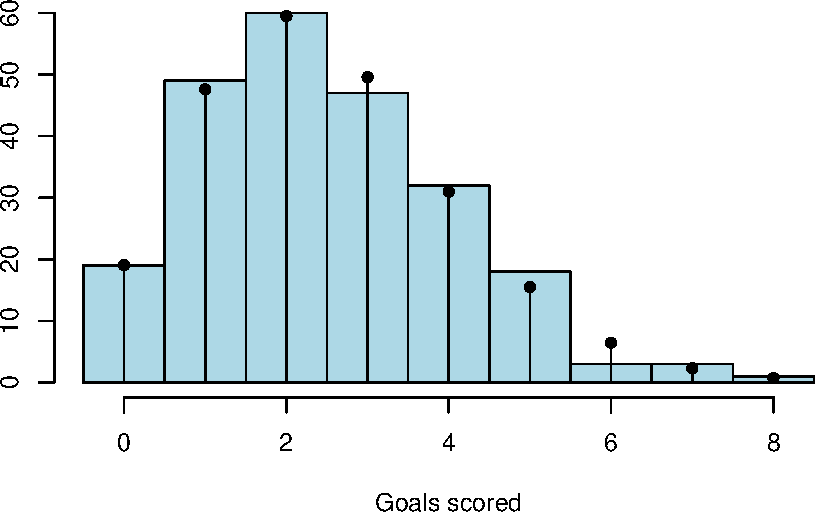
\includegraphics{SDM-CHAP22_files/figure-latex/histo-1} 

}

\caption{Histogram of observed goals for `SOCCER` with a superimposed Poisson distribution with lambda = 2.5 (vertical lines)}\label{fig:histo}
\end{figure}

\begin{center}\rule{0.5\linewidth}{0.5pt}\end{center}

Although the chi-square goodness-of-fit test is primarily designed for discrete distributions, it can also be used with a continuous distribution if appropriate categories are defined.

\begin{center}\rule{0.5\linewidth}{0.5pt}\end{center}

\hypertarget{example-1}{%
\subsubsection*{Example}\label{example-1}}
\addcontentsline{toc}{subsubsection}{Example}

Use the chi-square goodness-of-fit test with \(\alpha=0.05\) to test the hypothesis that the SAT scores stored in the data frame \texttt{GRADES} have a normal \textbf{cdf}. Use categories \((-\infty, \mu-2\sigma]\), \((\mu-2\sigma, \mu-\sigma]\), \((\mu-\sigma, \mu]\), \((\mu, \mu+\sigma]\), \((\mu+\sigma, \mu+2\sigma]\), and \((\mu+2\sigma, \infty]\). Produce a histogram using the categories specified and superimpose on the histogram the expected number of SAT scores in each category when \(F_0(x)\sim N(\mu=\bar{x}, \sigma=s)\).

\begin{center}\rule{0.5\linewidth}{0.5pt}\end{center}

\hypertarget{solution-1}{%
\subsubsection*{Solution}\label{solution-1}}
\addcontentsline{toc}{subsubsection}{Solution}

\textbf{Hypotheses}---The null and alternative hypotheses for using the chi-square goodness-of-fit test to test the hypothesis that the SAT scores stored in the data frame \texttt{GRADES} have a Normal \textbf{cdf} are

\begin{align*}
        H_0&: F_X(x) = F_0(x) \sim N(\mu=\bar{x},\, \sigma=s)\text{ for all } x \text{ versus
        }\\
        H_A&:  F_X(x) \ne F_0(x)\text{ for some } x.
\end{align*}

\textbf{Test Statistic}---Since the mean and standard deviation are unknown, the first step is to estimate the unknown parameters \(\mu\) and \(\sigma\) using \(\bar{x}=1134.65\) and \(s=145.6086774\).

\begin{Shaded}
\begin{Highlighting}[]
\NormalTok{mu }\OtherTok{\textless{}{-}} \FunctionTok{mean}\NormalTok{(GRADES}\SpecialCharTok{$}\NormalTok{sat)}
\NormalTok{sig }\OtherTok{\textless{}{-}} \FunctionTok{sd}\NormalTok{(GRADES}\SpecialCharTok{$}\NormalTok{sat) }
\FunctionTok{c}\NormalTok{(mu, sig)}
\end{Highlighting}
\end{Shaded}

\begin{verbatim}
[1] 1134.6500  145.6087
\end{verbatim}

Because a normal distribution is continuous, it is necessary to create categories that include all the data. The categories \(\mu - 3\sigma\) to \(\mu -2\sigma, \ldots, \mu +2\sigma\) to \(\mu + 3\sigma\) are 697.8239678 to 843.4326452, 843.4326452 to 989.0413226, 989.0413226 to 1134.65,
1134.65 to
1280.2586774, 1280.2586774 to 1425.8673548, and 1425.8673548 to 1571.4760322. These particular categories include all of the observed SAT scores; however, the probabilities actually computed for the largest and smallest categories will be all of the area to the right and left, respectively, of \(\bar{x} \pm 2s\). This is done so that the total area under the distribution in the null hypothesis is one.

\begin{Shaded}
\begin{Highlighting}[]
\NormalTok{bin }\OtherTok{\textless{}{-}} \FunctionTok{seq}\NormalTok{(}\AttributeTok{from =}\NormalTok{ mu }\SpecialCharTok{{-}} \DecValTok{3}\SpecialCharTok{*}\NormalTok{sig, }\AttributeTok{to =}\NormalTok{ mu }\SpecialCharTok{+} \DecValTok{3}\SpecialCharTok{*}\NormalTok{sig, }\AttributeTok{by =}\NormalTok{ sig)}
\FunctionTok{round}\NormalTok{(bin, }\DecValTok{0}\NormalTok{)                     }\CommentTok{\# vector of bin cut points}
\end{Highlighting}
\end{Shaded}

\begin{verbatim}
[1]  698  843  989 1135 1280 1426 1571
\end{verbatim}

\begin{Shaded}
\begin{Highlighting}[]
\NormalTok{T1 }\OtherTok{\textless{}{-}} \FunctionTok{table}\NormalTok{(}\FunctionTok{cut}\NormalTok{(GRADES}\SpecialCharTok{$}\NormalTok{sat, }\AttributeTok{breaks =}\NormalTok{ bin))}
\NormalTok{T1                                }\CommentTok{\# count of observations in bins}
\end{Highlighting}
\end{Shaded}

\begin{verbatim}
          (698,843]           (843,989]      (989,1.13e+03] (1.13e+03,1.28e+03] 
                  4                  27                  65                  80 
(1.28e+03,1.43e+03] (1.43e+03,1.57e+03] 
                 21                   3 
\end{verbatim}

\begin{Shaded}
\begin{Highlighting}[]
\NormalTok{OB }\OtherTok{\textless{}{-}} \FunctionTok{as.vector}\NormalTok{(T1)}
\NormalTok{OB                                }\CommentTok{\# vector of observations}
\end{Highlighting}
\end{Shaded}

\begin{verbatim}
[1]  4 27 65 80 21  3
\end{verbatim}

\begin{Shaded}
\begin{Highlighting}[]
\NormalTok{PR }\OtherTok{\textless{}{-}} \FunctionTok{c}\NormalTok{(}\FunctionTok{pnorm}\NormalTok{(}\SpecialCharTok{{-}}\DecValTok{2}\NormalTok{), }\FunctionTok{pnorm}\NormalTok{(}\SpecialCharTok{{-}}\DecValTok{1}\SpecialCharTok{:}\DecValTok{2}\NormalTok{) }\SpecialCharTok{{-}} \FunctionTok{pnorm}\NormalTok{(}\SpecialCharTok{{-}}\DecValTok{2}\SpecialCharTok{:}\DecValTok{1}\NormalTok{), }
        \FunctionTok{pnorm}\NormalTok{(}\DecValTok{2}\NormalTok{, }\AttributeTok{lower =} \ConstantTok{FALSE}\NormalTok{))  }\CommentTok{\# area under curve}
\NormalTok{EX }\OtherTok{\textless{}{-}} \DecValTok{200}\SpecialCharTok{*}\NormalTok{PR                      }\CommentTok{\# Expected count in bins}
\NormalTok{ans }\OtherTok{\textless{}{-}} \FunctionTok{cbind}\NormalTok{(PR, EX, OB)          }\CommentTok{\# column bind values in ans}
\NormalTok{ans}
\end{Highlighting}
\end{Shaded}

\begin{verbatim}
             PR        EX OB
[1,] 0.02275013  4.550026  4
[2,] 0.13590512 27.181024 27
[3,] 0.34134475 68.268949 65
[4,] 0.34134475 68.268949 80
[5,] 0.13590512 27.181024 21
[6,] 0.02275013  4.550026  3
\end{verbatim}

\textbf{Rejection Region Calculations}---Reject if \(\chi^2_{\text{obs}}>\chi^2_{1-\alpha;k-p-1}\). Now that the expected and observed counts for each of the categories are computed, the \(\chi_{\text{obs}}^2\) value can be computed according to \eqref{eq:chiobs} and is 4.1736536.

\begin{Shaded}
\begin{Highlighting}[]
\NormalTok{chi\_obs }\OtherTok{\textless{}{-}} \FunctionTok{sum}\NormalTok{((OB }\SpecialCharTok{{-}}\NormalTok{ EX)}\SpecialCharTok{\^{}}\DecValTok{2}\SpecialCharTok{/}\NormalTok{EX)}
\NormalTok{chi\_obs}
\end{Highlighting}
\end{Shaded}

\begin{verbatim}
[1] 4.173654
\end{verbatim}

\textbf{Statistical Conclusion}---In this problem, two parameters were estimated, and as a consequence, the degrees of freedom are computed as \(6-2-1=3\). The \(p-\)value is 0.2433129.

\begin{Shaded}
\begin{Highlighting}[]
\NormalTok{p\_val }\OtherTok{\textless{}{-}} \FunctionTok{pchisq}\NormalTok{(chi\_obs, }\DecValTok{6} \SpecialCharTok{{-}} \DecValTok{2} \SpecialCharTok{{-}} \DecValTok{1}\NormalTok{, }\AttributeTok{lower =} \ConstantTok{FALSE}\NormalTok{)}
\NormalTok{p\_val}
\end{Highlighting}
\end{Shaded}

\begin{verbatim}
[1] 0.2433129
\end{verbatim}

\begin{enumerate}
\def\labelenumi{\Roman{enumi}.}
\item
  Since \(\chi^2_{\text{obs}}=4.1736536\) is not greater than \(\chi^2_{0.95;3}=7.8147279\), fail to reject \(H_0\).
\item
  Since the \(p-\)value = 0.2433129 is greater than 0.05, fail to reject \(H_0\).
\end{enumerate}

\textbf{Fail to reject \(H_0\)}

\textbf{English Conclusion}---There is no evidence to suggest that the true \textbf{cdf} of SAT scores is not a normal distribution.

\begin{center}\rule{0.5\linewidth}{0.5pt}\end{center}

\textbf{Caution:}If one uses the \texttt{R} function \texttt{chisq.test()}, the degrees of
freedom and the subsequent \(p-\)value will be incorrect, as illustrated
below.

\begin{Shaded}
\begin{Highlighting}[]
\FunctionTok{chisq.test}\NormalTok{(}\AttributeTok{x =}\NormalTok{ OB, }\AttributeTok{p =}\NormalTok{ PR)  }\CommentTok{\# returns incorrect dof and p{-}value}
\end{Highlighting}
\end{Shaded}

\begin{verbatim}
    Chi-squared test for given probabilities

data:  OB
X-squared = 4.1737, df = 5, p-value = 0.5247
\end{verbatim}

Since it is not feasible to produce a histogram that extends from \(-\infty\) to \(\infty\), a histogram is created where the categories will simply cover the range of observed values. In this problem, the range of the SAT scores is 720 to 1550. The histogram with categories \((\mu-3\sigma, \mu-2\sigma]\), \((\mu-2\sigma, \mu-\sigma]\), \((\mu-\sigma, \mu]\), \((\mu+, \mu+\sigma]\), \((\mu+\sigma, \mu+2\sigma]\), and \((\mu+2\sigma, \mu+3\sigma]\), superimposed with the expected number of SAT scores for the categories \((-\infty, \mu-2\sigma]\), \((\mu-2\sigma, \mu-\sigma]\), \((\mu-\sigma, \mu]\), \((\mu, \mu+\sigma]\), \((\mu+\sigma, \mu+2\sigma]\), and \((\mu+2\sigma, \infty]\) is computed below and depicted in Figure \ref{fig:normsat}.

\begin{Shaded}
\begin{Highlighting}[]
\FunctionTok{hist}\NormalTok{(GRADES}\SpecialCharTok{$}\NormalTok{sat, }\AttributeTok{breaks =}\NormalTok{ bin, }\AttributeTok{col =} \StringTok{"lightblue"}\NormalTok{, }
     \AttributeTok{xlab =} \StringTok{"SAT scores"}\NormalTok{, }\AttributeTok{ylab=}\StringTok{""}\NormalTok{, }\AttributeTok{freq =} \ConstantTok{TRUE}\NormalTok{, }\AttributeTok{main =} \StringTok{""}\NormalTok{)}
\NormalTok{x }\OtherTok{\textless{}{-}}\NormalTok{ bin[}\DecValTok{2}\SpecialCharTok{:}\DecValTok{7}\NormalTok{] }\SpecialCharTok{{-}}\NormalTok{ sig}\SpecialCharTok{/}\DecValTok{2}
\NormalTok{fx }\OtherTok{\textless{}{-}}\NormalTok{ PR}\SpecialCharTok{*}\DecValTok{200}
\FunctionTok{lines}\NormalTok{(x, fx, }\AttributeTok{type =} \StringTok{"h"}\NormalTok{)}
\FunctionTok{lines}\NormalTok{(x, fx, }\AttributeTok{type =} \StringTok{"p"}\NormalTok{, }\AttributeTok{pch =} \DecValTok{16}\NormalTok{)}
\end{Highlighting}
\end{Shaded}

\begin{figure}

{\centering 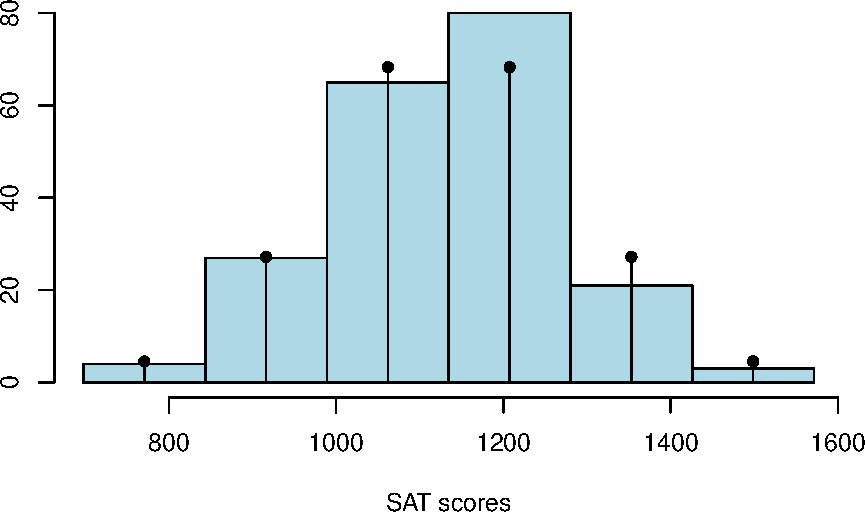
\includegraphics{SDM-CHAP22_files/figure-latex/normsat-1} 

}

\caption{Histogram of SAT scores in `Grades`}\label{fig:normsat}
\end{figure}

\begin{center}\rule{0.5\linewidth}{0.5pt}\end{center}

\textbf{Your Turn}

A psychology professor reports that historically grades in her intro class have been distributed
15\% A, 30\% B, 40\% C, 10\% D, and 5\% F. Grades this year were distributed:

\begin{verbatim}
  A   B   C   D   E 
 89 121  78  25  12 
\end{verbatim}

Is there evidence that this year's distribution is different from the historical distribution? If yes, which grade impacted that decision most?

\begin{Shaded}
\begin{Highlighting}[]
\CommentTok{\# Your Code Here}
\NormalTok{OB }\OtherTok{\textless{}{-}} \FunctionTok{c}\NormalTok{(}\DecValTok{89}\NormalTok{, }\DecValTok{121}\NormalTok{, }\DecValTok{78}\NormalTok{, }\DecValTok{25}\NormalTok{, }\DecValTok{12}\NormalTok{)}
\FunctionTok{names}\NormalTok{(OB) }\OtherTok{\textless{}{-}}\NormalTok{ LETTERS[}\DecValTok{1}\SpecialCharTok{:}\DecValTok{5}\NormalTok{]}
\NormalTok{OB}
\end{Highlighting}
\end{Shaded}

\begin{verbatim}
  A   B   C   D   E 
 89 121  78  25  12 
\end{verbatim}

\begin{Shaded}
\begin{Highlighting}[]
\NormalTok{EX }\OtherTok{\textless{}{-}} \FunctionTok{sum}\NormalTok{(OB)}\SpecialCharTok{*}\FunctionTok{c}\NormalTok{(}\FloatTok{0.15}\NormalTok{, }\FloatTok{0.3}\NormalTok{, }\FloatTok{0.4}\NormalTok{, }\FloatTok{0.1}\NormalTok{, }\FloatTok{0.05}\NormalTok{)}
\NormalTok{SS }\OtherTok{\textless{}{-}}\NormalTok{ (OB }\SpecialCharTok{{-}}\NormalTok{ EX)}\SpecialCharTok{\^{}}\DecValTok{2}\SpecialCharTok{/}\NormalTok{EX}
\NormalTok{SS}
\end{Highlighting}
\end{Shaded}

\begin{verbatim}
        A         B         C         D         E 
33.232051  5.664103 20.800000  1.730769  1.111538 
\end{verbatim}

\begin{Shaded}
\begin{Highlighting}[]
\CommentTok{\# Largest component is A\textquotesingle{}s}
\NormalTok{chi\_obs }\OtherTok{\textless{}{-}} \FunctionTok{sum}\NormalTok{(SS)}
\NormalTok{p\_val }\OtherTok{\textless{}{-}} \FunctionTok{pchisq}\NormalTok{(chi\_obs, }\DecValTok{4}\NormalTok{, }\AttributeTok{lower =} \ConstantTok{FALSE}\NormalTok{)}
\NormalTok{p\_val}
\end{Highlighting}
\end{Shaded}

\begin{verbatim}
[1] 8.48661e-13
\end{verbatim}

\begin{Shaded}
\begin{Highlighting}[]
\FunctionTok{chisq.test}\NormalTok{(}\AttributeTok{x =}\NormalTok{ OB, }\AttributeTok{p =} \FunctionTok{c}\NormalTok{(}\FloatTok{0.15}\NormalTok{, }\FloatTok{0.3}\NormalTok{, }\FloatTok{0.4}\NormalTok{, }\FloatTok{0.1}\NormalTok{, }\FloatTok{0.05}\NormalTok{))}
\end{Highlighting}
\end{Shaded}

\begin{verbatim}
    Chi-squared test for given probabilities

data:  OB
X-squared = 62.538, df = 4, p-value = 8.487e-13
\end{verbatim}

\begin{center}\rule{0.5\linewidth}{0.5pt}\end{center}

Given a contingency table (Question 5)

\begin{Shaded}
\begin{Highlighting}[]
\NormalTok{ad }\OtherTok{\textless{}{-}} \FunctionTok{c}\NormalTok{(}\DecValTok{20}\NormalTok{, }\DecValTok{45}\NormalTok{, }\DecValTok{35}\NormalTok{, }\DecValTok{25}\NormalTok{, }\DecValTok{50}\NormalTok{, }\DecValTok{25}\NormalTok{)}
\NormalTok{adm }\OtherTok{\textless{}{-}} \FunctionTok{matrix}\NormalTok{(ad, }\AttributeTok{byrow =} \ConstantTok{TRUE}\NormalTok{, }\AttributeTok{nrow =} \DecValTok{2}\NormalTok{)}
\NormalTok{adm}
\end{Highlighting}
\end{Shaded}

\begin{verbatim}
     [,1] [,2] [,3]
[1,]   20   45   35
[2,]   25   50   25
\end{verbatim}

\begin{Shaded}
\begin{Highlighting}[]
\FunctionTok{dimnames}\NormalTok{(adm) }\OtherTok{\textless{}{-}} \FunctionTok{list}\NormalTok{(}\AttributeTok{Branch =} \FunctionTok{c}\NormalTok{(}\StringTok{"In{-}Town"}\NormalTok{, }\StringTok{"Mall"}\NormalTok{), }\AttributeTok{Age =} \FunctionTok{c}\NormalTok{(}\StringTok{"Less Than 30"}\NormalTok{, }\StringTok{"30{-}55"}\NormalTok{, }\StringTok{"56 or older"}\NormalTok{))}
\NormalTok{adm}
\end{Highlighting}
\end{Shaded}

\begin{verbatim}
         Age
Branch    Less Than 30 30-55 56 or older
  In-Town           20    45          35
  Mall              25    50          25
\end{verbatim}

\begin{Shaded}
\begin{Highlighting}[]
\FunctionTok{chisq.test}\NormalTok{(adm)}
\end{Highlighting}
\end{Shaded}

\begin{verbatim}
    Pearson's Chi-squared test

data:  adm
X-squared = 2.4854, df = 2, p-value = 0.2886
\end{verbatim}

\begin{Shaded}
\begin{Highlighting}[]
\CommentTok{\# To get the expected counts use $exp}
\FunctionTok{chisq.test}\NormalTok{(adm)}\SpecialCharTok{$}\NormalTok{exp}
\end{Highlighting}
\end{Shaded}

\begin{verbatim}
         Age
Branch    Less Than 30 30-55 56 or older
  In-Town         22.5  47.5          30
  Mall            22.5  47.5          30
\end{verbatim}

To get \textbf{Standardized Residuals} compute \(\frac{(\text{Obs - Exp})}{\sqrt{\text{Exp}}}\). If using the \texttt{chisq.test()} function one may extract the residuals using \texttt{\$residuals}

\begin{Shaded}
\begin{Highlighting}[]
\FunctionTok{chisq.test}\NormalTok{(adm)}\SpecialCharTok{$}\NormalTok{residuals}
\end{Highlighting}
\end{Shaded}

\begin{verbatim}
         Age
Branch    Less Than 30      30-55 56 or older
  In-Town   -0.5270463 -0.3627381   0.9128709
  Mall       0.5270463  0.3627381  -0.9128709
\end{verbatim}

\begin{Shaded}
\begin{Highlighting}[]
\CommentTok{\# Equivalent to}
\NormalTok{(}\FunctionTok{chisq.test}\NormalTok{(adm)}\SpecialCharTok{$}\NormalTok{obs }\SpecialCharTok{{-}} \FunctionTok{chisq.test}\NormalTok{(adm)}\SpecialCharTok{$}\NormalTok{exp)}\SpecialCharTok{/}\FunctionTok{chisq.test}\NormalTok{(adm)}\SpecialCharTok{$}\NormalTok{exp}\SpecialCharTok{\^{}}\NormalTok{.}\DecValTok{5}
\end{Highlighting}
\end{Shaded}

\begin{verbatim}
         Age
Branch    Less Than 30      30-55 56 or older
  In-Town   -0.5270463 -0.3627381   0.9128709
  Mall       0.5270463  0.3627381  -0.9128709
\end{verbatim}

\textbf{Questions 8}

Given a ratio 9:3:3:1, the fraction for each category will be 9/16, 3/16, 3/16, 1/16.

\begin{Shaded}
\begin{Highlighting}[]
\NormalTok{obs }\OtherTok{\textless{}{-}} \FunctionTok{c}\NormalTok{(}\DecValTok{54}\NormalTok{, }\DecValTok{21}\NormalTok{, }\DecValTok{13}\NormalTok{, }\DecValTok{12}\NormalTok{)}
\NormalTok{obs2 }\OtherTok{\textless{}{-}}\NormalTok{ obs}\SpecialCharTok{*}\DecValTok{2}
\NormalTok{p }\OtherTok{\textless{}{-}} \FunctionTok{c}\NormalTok{(}\DecValTok{9}\SpecialCharTok{/}\DecValTok{16}\NormalTok{, }\DecValTok{3}\SpecialCharTok{/}\DecValTok{16}\NormalTok{, }\DecValTok{3}\SpecialCharTok{/}\DecValTok{16}\NormalTok{, }\DecValTok{1}\SpecialCharTok{/}\DecValTok{16}\NormalTok{)}
\FunctionTok{chisq.test}\NormalTok{(}\AttributeTok{x =}\NormalTok{ obs, }\AttributeTok{p =}\NormalTok{ p)}
\end{Highlighting}
\end{Shaded}

\begin{verbatim}
    Chi-squared test for given probabilities

data:  obs
X-squared = 7.4133, df = 3, p-value = 0.05983
\end{verbatim}

\begin{Shaded}
\begin{Highlighting}[]
\FunctionTok{chisq.test}\NormalTok{(obs2, }\AttributeTok{p =}\NormalTok{ p)}
\end{Highlighting}
\end{Shaded}

\begin{verbatim}
    Chi-squared test for given probabilities

data:  obs2
X-squared = 14.827, df = 3, p-value = 0.001971
\end{verbatim}

\begin{center}\rule{0.5\linewidth}{0.5pt}\end{center}

\hypertarget{independence-test}{%
\subsection{Independence test}\label{independence-test}}

\textbf{SCENARIO ONE:} Is there an association between gender and a person's happiness? To investigate whether happiness depends on gender, one might use information collected from the General Social Survey (GSS) \url{http://sda.berkeley.edu/GSS}. In each survey, the GSS asks, ``Taken all together, how would you say things are these days --- would you say that you are very happy, pretty happy, or not too happy?'\,' Respondents to each survey are coded as either male or female. The information below shows how a subset of respondents (26-year-olds) were classified with respect to the variables HAPPY and SEX.

\begin{Shaded}
\begin{Highlighting}[]
\NormalTok{HA }\OtherTok{\textless{}{-}} \FunctionTok{c}\NormalTok{(}\DecValTok{110}\NormalTok{, }\DecValTok{277}\NormalTok{, }\DecValTok{50}\NormalTok{, }\DecValTok{163}\NormalTok{, }\DecValTok{302}\NormalTok{, }\DecValTok{63}\NormalTok{)}
\NormalTok{HAT }\OtherTok{\textless{}{-}} \FunctionTok{matrix}\NormalTok{(}\AttributeTok{data =}\NormalTok{ HA, }\AttributeTok{nrow =} \DecValTok{2}\NormalTok{, }\AttributeTok{byrow =} \ConstantTok{TRUE}\NormalTok{)}
\FunctionTok{dimnames}\NormalTok{(HAT) }\OtherTok{\textless{}{-}} \FunctionTok{list}\NormalTok{(}\AttributeTok{SEX =} \FunctionTok{c}\NormalTok{(}\StringTok{"Male"}\NormalTok{, }\StringTok{"Female"}\NormalTok{),}
    \AttributeTok{Category =} \FunctionTok{c}\NormalTok{(}\StringTok{"Very Happy"}\NormalTok{, }\StringTok{"Pretty Happy"}\NormalTok{, }\StringTok{"Not To Happy"}\NormalTok{))}
\NormalTok{HAT}
\end{Highlighting}
\end{Shaded}

\begin{verbatim}
        Category
SEX      Very Happy Pretty Happy Not To Happy
  Male          110          277           50
  Female        163          302           63
\end{verbatim}

Scenario one asks if there is an association between gender and a person's happiness. Two events, \(A\) and \(B\), were defined as independent when \(P(A \cap B)=P(A)\times P(B)\) or, equivalently, when \(P(A|B)=P(A)\). If, instead of having a random sample from a single population, an \(I \times J\) contingency table consisted of entries from the population, association could be mathematically verified by showing that \(P(n_{ij}) \ne P(n_{i\bullet}) \times P(n_{\bullet j})\) for some \(i\) and \(j\). If by chance \(P(n_{ij}) = P(n_{i\bullet}) \times P(n_{\bullet j})\) for all \(i\) and \(j\), then one would conclude there is no association between gender and a person's happiness. That is, the variables gender and happiness would be considered mathematically independent. Since the entire population is not given but rather a sample from a population, the values in the \(I \times J\) contingency table can be expected to change from sample to sample. The question is, ``By how much can the variables deviate from the mathematical definition of independence and still be considered statistically independent?'\,'

The null and alternative hypotheses to test for independence between row and column variables is written \(H_0: \pi_{ij}=\pi_{i\bullet}\pi_{\bullet j}\) versus \(H_A:\pi_{ij} \ne \pi_{i\bullet}\pi_{\bullet j}\). The test statistic is

\begin{equation}
\chi_{\text{obs}}^2 =\sum_{i=1}^I\sum_{j=1}^J \frac{(O_{ij} - E_{ij})^2}{E_{ij}}
\label{eq:ChiSqStatIndep}
\end{equation}

It compares the observed frequencies in the table with the expected frequencies when \(H_0\) is true. Under the assumption of independence, and when the observations in the cells are sufficiently large (usually greater than 5), \(\chi_{\text{obs}}^2 =\sum_{i=1}^{I}\sum_{j=1}^J \frac{(n_{ij}-\hat{\mu}_{ij})^2}{\hat{\mu}_{ij}} \overset{\bullet}{\sim} \chi^2_{(I-1)(J-1)},\) where \(\hat{\mu}_{ij}=\frac{n_{i\bullet}n_{\bullet j}}{n} = E_{ij}\) and \(n_{ij} = O_{ij}\). The null hypothesis of independence is rejected when \(\chi_{\text{obs}}^2 > \chi^2_{1-\alpha; (I-1)(J-1)}\).

The chi-squared approximation is generally satisfactory if the \(E_{ij}\)s (\(\hat{\mu}_{ij}\)s) in the test statistic are not too small. Various rules of thumb exist for what might be considered too small. A very conservative rule is to require all \(E_{ij}\)s to be 5 or more. This can be accomplished by combining cells with small \(E_{ij}\)s and reducing the overall degrees of freedom. At times, it may be permissible to let the \(E_{ij}\) of a cell be as low as 0.5.

\begin{center}\rule{0.5\linewidth}{0.5pt}\end{center}

\textbf{Test For SCENARIO ONE:}

\textbf{Hypotheses} --- \(H_0: \pi_{ij} = \pi_{i\bullet }\pi_{\bullet j}\)
(Row and column variables are independent.)
versus \(H_A: \pi_{ij} \ne \pi_{i\bullet }\pi_{\bullet j}\) for at least one \(i, j\)
(Row and column variables are dependent.)

\textbf{Test Statistic} --- The test statistic is
\[\chi_{\text{obs}}^2=\sum_{i=1}^I \sum_{j=1}^J 
        \frac{(O_{ij}-E_{ij})^2}{E_{ij}} \overset{\bullet}{\sim} \chi^2_{(I-1)(J-1)}=
        \chi^2_{(2-1)(3-1)}=\chi^2_2\]
under the assumption of independence. The \(\chi^2_{\text{obs}}\) value is
\(4.3214818\).

\begin{Shaded}
\begin{Highlighting}[]
\FunctionTok{chisq.test}\NormalTok{(HAT)}\SpecialCharTok{$}\NormalTok{stat}
\end{Highlighting}
\end{Shaded}

\begin{verbatim}
X-squared 
 4.321482 
\end{verbatim}

\textbf{Rejection Region Calculations} --- The rejection region is \[\chi_{\text{obs}}^2 > \chi^2_{1-\alpha; (I-1)(J-1)}=\chi^2_{0.95;2}= 5.9914645.\] Before the statistic \(\chi^2_{\text{obs}}= \sum_{i=1}^I\sum_{j=1}^J \frac{(O_{ij} - E_{ij})^2}{E_{ij}}\) can be computed, the expected counts for each of the \(ij\) cells must be calculated. Note that \(O_{ij}=n_{ij}\) and \(E_{ij}=\frac{n_{i\bullet}n_{\bullet j}}{n}\).

\begin{Shaded}
\begin{Highlighting}[]
\NormalTok{E }\OtherTok{\textless{}{-}} \FunctionTok{chisq.test}\NormalTok{(HAT)}\SpecialCharTok{$}\NormalTok{exp}
\NormalTok{E}
\end{Highlighting}
\end{Shaded}

\begin{verbatim}
        Category
SEX      Very Happy Pretty Happy Not To Happy
  Male      123.628        262.2     51.17202
  Female    149.372        316.8     61.82798
\end{verbatim}

\[\chi^2_{\text{obs}}=\frac{(110 - 123.6280)^2}{123.6280} +
\frac{(277-262.2)^2}{262.2}+ \dots +\frac{(63-61.828)^2}{61.828}=4.3215.\]

The value of the test statistic is \(\chi^2_{obs}= 4.3214818\).
This can be done with code by entering

\begin{Shaded}
\begin{Highlighting}[]
\FunctionTok{chisq.test}\NormalTok{(HAT)}\SpecialCharTok{$}\NormalTok{stat}
\end{Highlighting}
\end{Shaded}

\begin{verbatim}
X-squared 
 4.321482 
\end{verbatim}

\begin{Shaded}
\begin{Highlighting}[]
\CommentTok{\# Or}
\NormalTok{chi\_obs }\OtherTok{\textless{}{-}} \FunctionTok{sum}\NormalTok{((HAT }\SpecialCharTok{{-}}\NormalTok{ E)}\SpecialCharTok{\^{}}\DecValTok{2}\SpecialCharTok{/}\NormalTok{E)}
\NormalTok{chi\_obs}
\end{Highlighting}
\end{Shaded}

\begin{verbatim}
[1] 4.321482
\end{verbatim}

\(4.3214818 = \chi^2_{\text{obs}} \overset{?}{>} \chi^2_{0.95,2}= 5.9914645\).

\textbf{Statistical Conclusion} --- The \(p-\)value is 0.1152397

\begin{Shaded}
\begin{Highlighting}[]
\FunctionTok{chisq.test}\NormalTok{(HAT)}
\end{Highlighting}
\end{Shaded}

\begin{verbatim}
    Pearson's Chi-squared test

data:  HAT
X-squared = 4.3215, df = 2, p-value = 0.1152
\end{verbatim}

\begin{Shaded}
\begin{Highlighting}[]
\FunctionTok{chisq.test}\NormalTok{(HAT)}\SpecialCharTok{$}\NormalTok{p.value}
\end{Highlighting}
\end{Shaded}

\begin{verbatim}
[1] 0.1152397
\end{verbatim}

\begin{Shaded}
\begin{Highlighting}[]
\CommentTok{\# Or}
\NormalTok{p\_val }\OtherTok{\textless{}{-}} \FunctionTok{pchisq}\NormalTok{(chi\_obs, }\DecValTok{2}\NormalTok{, }\AttributeTok{lower =} \ConstantTok{FALSE}\NormalTok{)}
\NormalTok{p\_val}
\end{Highlighting}
\end{Shaded}

\begin{verbatim}
[1] 0.1152397
\end{verbatim}

\begin{enumerate}
\def\labelenumi{\Roman{enumi}.}
\item
  From the rejection region, since \(\chi_{\text{obs}}^2=4.3214818 < \chi^2_{0.95;2}=5.9914645\). fail to reject the null hypothesis of independence.
\item
  Since the \(p-\)value = \(0.1152397\) is greater than 0.05, fail to reject the null hypothesis of independence.
\end{enumerate}

\textbf{Fail to reject \(H_0\).}

\textbf{English Conclusion} --- There is not sufficient evidence to suggest the variables gender and happiness are statistically dependent.

\begin{center}\rule{0.5\linewidth}{0.5pt}\end{center}

\hypertarget{example-2}{%
\subsubsection*{EXAMPLE}\label{example-2}}
\addcontentsline{toc}{subsubsection}{EXAMPLE}

Is there an association between eye color and hearing loss in patients suffering from meningitis? British researcher \href{}{Helen Cullingham} recorded the eye color of 130 deaf patients and noted whether the deafness had followed treatment for meningitis.

\begin{Shaded}
\begin{Highlighting}[]
\NormalTok{HC }\OtherTok{\textless{}{-}} \FunctionTok{c}\NormalTok{(}\DecValTok{30}\NormalTok{, }\DecValTok{72}\NormalTok{, }\DecValTok{2}\NormalTok{, }\DecValTok{26}\NormalTok{)}
\NormalTok{HCM }\OtherTok{\textless{}{-}} \FunctionTok{matrix}\NormalTok{(HC, }\AttributeTok{byrow =} \ConstantTok{TRUE}\NormalTok{, }\AttributeTok{nrow =} \DecValTok{2}\NormalTok{)}
\FunctionTok{dimnames}\NormalTok{(HCM) }\OtherTok{\textless{}{-}} \FunctionTok{list}\NormalTok{(}\AttributeTok{Eye\_Color =} \FunctionTok{c}\NormalTok{(}\StringTok{"Light"}\NormalTok{, }\StringTok{"Dark"}\NormalTok{), }\AttributeTok{Deafness\_related\_to =} \FunctionTok{c}\NormalTok{(}\StringTok{"Meningitis"}\NormalTok{, }\StringTok{"Other"}\NormalTok{))}
\NormalTok{HCM}
\end{Highlighting}
\end{Shaded}

\begin{verbatim}
         Deafness_related_to
Eye_Color Meningitis Other
    Light         30    72
    Dark           2    26
\end{verbatim}

\begin{Shaded}
\begin{Highlighting}[]
\CommentTok{\#Your code to test the appropriate hypothesis}

\FunctionTok{chisq.test}\NormalTok{(HCM, }\AttributeTok{correct =} \ConstantTok{FALSE}\NormalTok{)}
\end{Highlighting}
\end{Shaded}

\begin{verbatim}
    Pearson's Chi-squared test

data:  HCM
X-squared = 5.8712, df = 1, p-value = 0.01539
\end{verbatim}

\begin{center}\rule{0.5\linewidth}{0.5pt}\end{center}

\textbf{SCENARIO TWO:} In a double blind randomized drug trial (neither the patient nor the physician evaluating the patient knows the treatment, drug or placebo, the patient receives), 400 male patients with mild dementia were randomly divided into two groups of 200. One group was given a placebo over three months while the second group received an experimental drug for three months. At the end of the three months, the physicians (all psychiatrists) classified the 400 patients into one of three categories: improved, no change, or worse. The information below shows how the psychiatrists classified the patients. Are the proportions in the three status categories the same for the two treatments?

\begin{Shaded}
\begin{Highlighting}[]
\NormalTok{DT }\OtherTok{\textless{}{-}} \FunctionTok{c}\NormalTok{(}\DecValTok{67}\NormalTok{, }\DecValTok{76}\NormalTok{, }\DecValTok{57}\NormalTok{, }\DecValTok{48}\NormalTok{, }\DecValTok{73}\NormalTok{, }\DecValTok{79}\NormalTok{)}
\NormalTok{DTT }\OtherTok{\textless{}{-}} \FunctionTok{matrix}\NormalTok{(}\AttributeTok{data =}\NormalTok{ DT, }\AttributeTok{nrow =} \DecValTok{2}\NormalTok{, }\AttributeTok{byrow =} \ConstantTok{TRUE}\NormalTok{)}
\FunctionTok{dimnames}\NormalTok{(DTT) }\OtherTok{\textless{}{-}} \FunctionTok{list}\NormalTok{(}\AttributeTok{Treatment =} \FunctionTok{c}\NormalTok{(}\StringTok{"Drug"}\NormalTok{, }\StringTok{"Placebo"}\NormalTok{),}
   \AttributeTok{Category =} \FunctionTok{c}\NormalTok{(}\StringTok{"Improve"}\NormalTok{, }\StringTok{"No Change"}\NormalTok{, }\StringTok{"Worse"}\NormalTok{))}
\NormalTok{DTT}
\end{Highlighting}
\end{Shaded}

\begin{verbatim}
         Category
Treatment Improve No Change Worse
  Drug         67        76    57
  Placebo      48        73    79
\end{verbatim}

In the \textbf{second scenario}, there are two distinct populations from which samples are taken. The first population is the group of all patients receiving the experimental drug while the second population is the group of all patients receiving a placebo. In this scenario, there are \(I=2\) separate populations and \(J=3\) categories for the \(I=2\) populations. Individuals sampled from the \(I=2\) distinct populations are classified into one of the \(J=3\) status categories. This scenario has fixed row totals whereas the \textbf{first scenario} does not. In the first scenario, only the total sample size, \(n\), is fixed. That is, neither the row nor the column totals are fixed. This is in contrast to \textbf{scenario two}, where the number of patients in each treatment group (row) was fixed.

\hypertarget{test-of-homogeneity}{%
\subsection{Test of Homogeneity}\label{test-of-homogeneity}}

The question of interest in \textbf{scenario two} is whether the proportions in each of the \(j=3\) categories for the \(i=2\) populations are equivalent. Specifically, is \(\pi_{1j} = \pi_{2j}\) for all \(j\)? This question is answered with a test of homogeneity. In general, the null hypothesis for a test of homogeneity with \(i=I\) populations is written

\begin{equation}
 H_0: \pi_{1j}=\pi_{2j} = \dots = \pi_{Ij}\text{ for all } j \text{ versus } H_1:
\pi_{ij} \ne \pi_{i+1, j} \: \text{ for some } (i, j).
\end{equation}

Expressed in words, the null hypothesis is that the \(I\) populations are
homogeneous with respect to the \(J\) categories versus the \(I\) populations are not homogeneous with respect to the \(J\) categories.

An equivalent interpretation is that for each population \(i=1,2,\dots, I\), the proportion of people in the \(j\text{th}\) category is the same. When \(H_0\) is true, \(\pi_{1j}=\pi_{2j}=\dots=\pi_{Ij}\) for all \(j\). Under the null hypothesis, \(\mu_{ij}= n_{i\bullet} \pi_{ij}\), \(\hat\pi_{ij}=p_{ij}= \frac{n_{\bullet j}}{n_{\bullet\bullet}}\), and \(\hat{\mu}_{ij}= \frac{n_{i\bullet} n_{\bullet j}}{n_{\bullet\bullet}}=E_{ij}\). When \(H_0\) is true, all the probabilities in the \(j\)\text{th} column are equal, and a pooled estimate of \(\pi_{ij}\) is obtained by adding all the frequencies in the \(j\)\text{th} column \((n_{\bullet j})\) and dividing the total by \(n_{\bullet\bullet}\). The statistic used in this type of problem has the same form as the one used for the test of independence in \eqref{eq:ChiSqStatIndep}. Substituting the homogeneity expressions for \(O_{ij}\) and \(E_{ij}\), the statistic is expressed as

\[\chi_{\text{obs}}^2=\sum_{i=1}^I\sum_{j=1}^J \frac{(n_{ij} - n_{i\bullet} n_{\bullet
j}/n_{\bullet\bullet})^2}{n_{i\bullet} n_{\bullet j}/n_{\bullet\bullet}} \overset{\cdot}{\sim}
\chi^2_{(I-1)(J-1)}.\] The null hypothesis of homogeneity is rejected when
\(\chi_{\text{obs}}^2 > \chi^2_{1-\alpha; (I-1)(J-1)}\).

\begin{center}\rule{0.5\linewidth}{0.5pt}\end{center}

\textbf{Test for SCENARIO TWO:}

\textbf{Hypotheses}--- \(H_0: \pi_{1j}=\pi_{2j} \text{ for all } j\) versus \(H_A: \pi_{i,\, j} \ne \pi_{i+1,\, j}\text{ for some }(i, j)\). That is, all the probabilities in the same column are equal to each other versus at least two of the probabilities in the same column are not equal to each other.

\textbf{Test Statistic}---The test statistic is
\[\chi_{\text{obs}}^2=\sum_{i=1}^I \sum_{j=1}^J 
        \frac{(O_{ij}-E_{ij})^2}{E_{ij}} \sim \chi^2_{(I-1)(J-1)}=
        \chi^2_{(2-1)(3-1)}=\chi^2_2\]
under the null hypothesis. The \(\chi^2_{\text{obs}}\) value is
\(6.7583566\).

\textbf{Rejection Region Calculations}---The rejection region is
\[\chi_{\text{obs}}^2 > \chi^2_{1-\alpha; (I-1)\cdot(J-1)} = 
        \chi^2_{0.95;2}=5.9914645.\]\\
Before the statistic \(\chi^2_{\text{obs}}= \sum_{i=1}^I\sum_{j=1}^J \frac{(O_{ij} - E_{ij})^2}{E_{ij}}\) can be computed, the expected counts for each of the \(ij\) cells must be determined. Recall that \(O_{ij}=n_{ij}\) and \(E_{ij}=\frac{n_{i\bullet}n_{\bullet j}}{n_{\bullet\bullet}}.\)

\begin{Shaded}
\begin{Highlighting}[]
\NormalTok{DTT}
\end{Highlighting}
\end{Shaded}

\begin{verbatim}
         Category
Treatment Improve No Change Worse
  Drug         67        76    57
  Placebo      48        73    79
\end{verbatim}

\begin{Shaded}
\begin{Highlighting}[]
\NormalTok{E }\OtherTok{\textless{}{-}} \FunctionTok{chisq.test}\NormalTok{(DTT)}\SpecialCharTok{$}\NormalTok{expected}
\NormalTok{E}
\end{Highlighting}
\end{Shaded}

\begin{verbatim}
         Category
Treatment Improve No Change Worse
  Drug       57.5      74.5    68
  Placebo    57.5      74.5    68
\end{verbatim}

\[\chi^2_{\text{obs}}=\frac{(67 - 57.5)^2}{57.5} + \frac{(76 - 74.5)^2}{74.5}+
\dots +\frac{(79-68)^2}{68}=6.7583566.\]

The value of the test statistic is \(\chi^2_{obs}=6.7583566.\) This can be done with code by entering

\begin{Shaded}
\begin{Highlighting}[]
\FunctionTok{chisq.test}\NormalTok{(DTT)}
\end{Highlighting}
\end{Shaded}

\begin{verbatim}
    Pearson's Chi-squared test

data:  DTT
X-squared = 6.7584, df = 2, p-value = 0.03408
\end{verbatim}

\begin{Shaded}
\begin{Highlighting}[]
\FunctionTok{chisq.test}\NormalTok{(DTT)}\SpecialCharTok{$}\NormalTok{stat}
\end{Highlighting}
\end{Shaded}

\begin{verbatim}
X-squared 
 6.758357 
\end{verbatim}

\begin{Shaded}
\begin{Highlighting}[]
\CommentTok{\# Or }
\NormalTok{chi\_obs }\OtherTok{\textless{}{-}} \FunctionTok{sum}\NormalTok{((DTT }\SpecialCharTok{{-}}\NormalTok{ E)}\SpecialCharTok{\^{}}\DecValTok{2}\SpecialCharTok{/}\NormalTok{E)}
\NormalTok{chi\_obs}
\end{Highlighting}
\end{Shaded}

\begin{verbatim}
[1] 6.758357
\end{verbatim}

\(6.7583566 = \chi^2_{\text{obs}}\overset{?}{>} \chi^2_{.95,2}= 5.9914645.\)

\textbf{Statistical Conclusion}---The \(p-\)value is \(0.0340754.\)

\begin{Shaded}
\begin{Highlighting}[]
\NormalTok{p\_val }\OtherTok{\textless{}{-}} \FunctionTok{pchisq}\NormalTok{(chi\_obs, }\DecValTok{2}\NormalTok{, }\AttributeTok{lower =} \ConstantTok{FALSE}\NormalTok{)}
\NormalTok{p\_val}
\end{Highlighting}
\end{Shaded}

\begin{verbatim}
[1] 0.03407544
\end{verbatim}

\begin{enumerate}
\def\labelenumi{\Roman{enumi}.}
\item
  From the rejection region, since \(\chi_{\text{obs}}^2= 6.7583566 > \chi_{0.95;2} = 5.9914645\), reject the null hypothesis of homogeneity.
\item
  Since the \(p-\)value = \(0.0340754\) is less than 0.05,
  reject the null hypothesis of homogeneity.
\end{enumerate}

\textbf{Reject \(H_0\).}

\textbf{English Conclusion}---There is sufficient evidence to suggest that not all of the probabilities for the \(i=2\) populations with respect to each of the \(J\) categories are equal.

\begin{center}\rule{0.5\linewidth}{0.5pt}\end{center}

\hypertarget{example-3}{%
\subsection*{Example}\label{example-3}}
\addcontentsline{toc}{subsection}{Example}

In a study of the television viewing havits of children, a developmental psychologist selects two random samples of first graders: one with 100 boys and one with 200 girls. Each child is asked which of the following TV programs the like best: The Lone Ranger, Sesame Street, or The Simpsons. Results are shown below.

\begin{Shaded}
\begin{Highlighting}[]
\NormalTok{TV }\OtherTok{\textless{}{-}} \FunctionTok{c}\NormalTok{(}\DecValTok{50}\NormalTok{, }\DecValTok{30}\NormalTok{, }\DecValTok{20}\NormalTok{, }\DecValTok{50}\NormalTok{, }\DecValTok{80}\NormalTok{, }\DecValTok{70}\NormalTok{)}
\NormalTok{TVM }\OtherTok{\textless{}{-}} \FunctionTok{matrix}\NormalTok{(}\AttributeTok{data =}\NormalTok{ TV, }\AttributeTok{nrow =} \DecValTok{2}\NormalTok{, }\AttributeTok{byrow =} \ConstantTok{TRUE}\NormalTok{)}
\FunctionTok{dimnames}\NormalTok{(TVM) }\OtherTok{\textless{}{-}} \FunctionTok{list}\NormalTok{(}\AttributeTok{FirstGraders =} \FunctionTok{c}\NormalTok{(}\StringTok{"Boys"}\NormalTok{, }\StringTok{"Girls"}\NormalTok{), }\AttributeTok{ViewingPreference =} \FunctionTok{c}\NormalTok{(}\StringTok{"Lone Ranger"}\NormalTok{, }\StringTok{"Sesame Street"}\NormalTok{, }\StringTok{"The Simpsons"}\NormalTok{))}
\NormalTok{TVM}
\end{Highlighting}
\end{Shaded}

\begin{verbatim}
            ViewingPreference
FirstGraders Lone Ranger Sesame Street The Simpsons
       Boys           50            30           20
       Girls          50            80           70
\end{verbatim}

Do the boys' preferences for these TV programs differ significantly from the girls' preferences? Use \(\alpha= 0.05\) to test your hypotheses.

\begin{Shaded}
\begin{Highlighting}[]
\FunctionTok{chisq.test}\NormalTok{(TVM)}
\end{Highlighting}
\end{Shaded}

\begin{verbatim}
    Pearson's Chi-squared test

data:  TVM
X-squared = 19.318, df = 2, p-value = 6.384e-05
\end{verbatim}

\textbf{Your English Conclusion}

\begin{center}\rule{0.5\linewidth}{0.5pt}\end{center}

\hypertarget{what-can-go-wrong}{%
\subsubsection*{What can go wrong?}\label{what-can-go-wrong}}
\addcontentsline{toc}{subsubsection}{What can go wrong?}

\begin{enumerate}
\def\labelenumi{\arabic{enumi}.}
\tightlist
\item
  \(\chi^2\) tests are \textbf{only} for counts
\item
  Samples reasonably sized
\item
  Note that ``not independent'' \(\neq\) dependent, only association exists
\end{enumerate}

\begin{center}\rule{0.5\linewidth}{0.5pt}\end{center}

\end{document}
